%%
%% 2019 07 04 Ph. G. Freimann
%%
\section{Quadratische Gleichungen\TALS{ I}}\index{Gleichungen!quadratische}
\sectuntertitel{Psychiater zur Quadratischen: ``Auch für
  Dich finden wir die eine oder andere Lösung.''}

%%\GESOTadBMTA{165}{10}
%%\TALSTadBFWA{93}{2.3}
\TadBMTA{165}{10}

%%%%%%%%%%%%%%%%%%%%%%%%%%%%%%%%%%%%%%%%%%%%%%%%%%%%%%%%%%%%%%%%%%%%%%%%%%%%%%%%%
\subsection*{Lernziele}

\begin{itemize}
\item Grundform $ax^2+bx+c=0$
\item Lösungsmethoden 
\item Allgemeine Form, ABC-Formel (Mitternachtsformel) $x_{1,2} = \frac{-b \pm \sqrt{b^2-4ac}}{2a} $
%%   \item Rationale Gleichungen (<- die Bruchgleichungen haben ein eigenes Kapitel)
\item Diskriminante
\TALS{\item{Parameter}}
\TALS{\item{Fallunterscheidung}}
\item Taschenrechner: \GESO{Ohne Parameter} \TALS{Mit und ohne Parameter}
\TALS{\item Taschenrechner: Visualisierung, Interpretation}
\end{itemize}
\newpage
\TRAINER{Typische Hausaufgabe als Einstieg:}
\subsection{Einstieg}
\subsubsection{Einstiegsaufgabe Snapchat}\index{Snapchat}
\aufgabenFarbe{In einem Campus werden innerhalb eines W-LANs
  29\,501\,192 bestimmte Datenpakete der ganzen Schule registriert. Wir gehen davon aus, dass dabei jede Person
genau ein \textit{snap} an alle anderen versendet hat.\\Wie viele Personen waren
beteiligt?}

Lösung:
\TNT{0.8}{$5432$ Personen (waren beteiligt).}

Lösungsstrategien:

\TNTeop{
  Wie sieht es bei $3$ Personen aus?
  Alle $3$ senden es $2$ Personen weiter.

  $$3\cdot{}2 = 6\text{ snaps}$$
Wie sieht es bei 10 Personen aus?
  $$10\cdot{}9 = 90$$

  Es sollen aber $29\,501\,192$ sein.
  
  $n$ sei die Anzahl Schüler.

  Jeder sendet $n-1$ Post; d.\,h. es werden $n\cdot{}(n-1)$ Posts
  versendet.

  Gleichung:

  $$n\cdot{}(n-1) = 29501192 \Longrightarrow   n^2 - n = 295011292 \text{ =
    quadratische Gleichung}$$

  Die Lösung $5432$ kann \zB durch ein Ausprobieren ermittelt werden.
  
  Das Ausprobieren könnte noch durch $\sqrt{29501192}\approx 5431$  angenähert werden;
  als ersten Startwert.

  Hier ev. noch die Lösung des openai.com chats (GPT chatbot) zeigen.
}

\newpage

\GESO{%%

%% Voraussetzungen fürs Verständnis der quadratischen Gleichungen

\subsection{Voraussetzungen / Repetition}
\TRAINER{selbständig\\}
A) Berechnen Sie:

$$(-5)\cdot{}(-5) = \LoesungsRaum{+25}$$

B) Faktorisieren Sie:

$$x^2-12x+36$$

\TNT{6}{
  Binomische Formeln

  $$x^2-12x+36 = (x-6)\cdot{}(x-6)=(x-6)^2$$
}


C) Finden Sie die Lösungsmenge für die Variable $x$:

$$|x-2| = 7$$

\TNTeop{a) $x-2 = 7$

  b) $x-2=-7 \Longrightarrow |x-2| = 7$

  $$\lx = \{-5; 9\}$$

}


\newpage
}
\TALS{%%

%% Voraussetzungen fürs Verständnis der quadratischen Gleichungen

\subsection{Voraussetzungen / Repetition}
\TRAINER{selbständig\\}
A) Berechnen Sie:

$$(-5)\cdot{}(-5) = \LoesungsRaum{+25}$$

B) Faktorisieren Sie:

$$x^2-12x+36$$

\TNT{6}{
  Binomische Formeln

  $$x^2-12x+36 = (x-6)\cdot{}(x-6)=(x-6)^2$$
}


C) Finden Sie die Lösungsmenge für die Variable $x$:

$$|x-2| = 7$$

\TNTeop{a) $x-2 = 7$

  b) $x-2=-7 \Longrightarrow |x-2| = 7$

  $$\lx = \{-5; 9\}$$

}


\newpage
}

\newpage

\subsubsection{Erste quadratische Gleichungen}
\TRAINER{Einzelarbeit; danach geführt Lösungsweg gemeinsam festhalten.}
$$x^2=49$$

\TNT{6}{

  $$ \left(
  \begin{bbwFillInTabular}{c}
  $\sqrt{x^2} = \sqrt{49}$\\
     $\TALS{|x| = 7}\GESO{x=\pm\sqrt{49}}$\\
  $x=7\text{ oder } x=-7$
    \end{bbwFillInTabular}
  \right) \text{Notation: } | \pm \sqrt{} \, {\color{red}\pm! \text{ nicht vergessen!}}$$
  
  $$x=\pm 7$$
  
  $\lx = \{-7; 7\}$ \vspace{15mm}
}%% END TNT

\TRAINER{\hrule}

$$(x-2)^2=49$$

\TNTeop{
\TALS{
( Erinnert Sie das ursprüngliche Beispiel an $|x-2| = 7$ ??)
}%% end TALS

  Direkt Wurzel ziehen:

  $$\left(
  \begin{bbwFillInTabular}{c}
    $ \sqrt{(x-2)^2}= \sqrt{49}$\\
        $\TALS{|x-2|=7}\GESO{x-2 = \pm\sqrt{49}}$\\
    $(x-2) = 7 \text{ od. } (x-2)= -7$
  \end{bbwFillInTabular} 
  \right) |  {\color{red}(\pm)} \, \sqrt{}$$
  
 $$x-2=\pm 7$$
 $$x=2\pm7$$

 $$\lx = \{-5; 9\}$$


  
  danach unbedingt Probe vorzeigen:

  $$x_1 = -5: (-5-2)^2 = (-7)^2 = 49$$
  $$x_2 = 9: (9-2)^2 = (7)^2 = 49$$

}%% END TNT


\newpage
%%%%%%%%%%%%%%%%%%%%%%%%%%%%%%%%%%%%%%%%%%%%%%%%%%%%%%%%%%%%%%%%%%%

%%\TRAINER{Normalform $x^2 +5x +6 = 0 \rightarrow (x+2)(x+3)=0$}
%%\newpage

%% \TALS{%% Vorbereitungsaufgaben zur quadratischen Ergänzung
%%  Stil x² + 2bx + b² = Zahl
%%

\subsection*{Aufgaben}

\TRAINER{Zweireteams/Bankreihen}

Geben Sie jeweils die Lösungsmenge $\mathbb{L}$ an:

$$x^2 = 7$$

\TNT{4}{$\lx = \{-\sqrt{7}; \sqrt{7}\}$}


$$(x+6)^2 = 3$$

\TNT{3.2}{$x-6=\pm\sqrt{3}$\\
  $x=6\pm\sqrt{3}$\\
  $\lx = \{6-\sqrt{3}; 6+\sqrt{3}\}$}


$$(x-5)^2 = 0$$

\TNT{3.2}{
  $x-5=\pm\sqrt{0} = 0$\\
  $x=5$\\
  $\lx = \{5\}$}



$$(x-5)^2 = -9$$

\TNT{4}{
  $x-5=\pm\sqrt{-9} ???$\\
  $\lx = \{\}$}


\newpage
$$(x+3)^2 = 2$$

\TNT{4}{
$x+3 = \pm\sqrt{2}$\\
$x=-3\pm\sqrt{2}$\\
  $\lx = \{-3-\sqrt{2}; -3+\sqrt{2}\}$}


$$x^2 + 6x + 9 = 2$$

\TNT{4}{
  $(x+3)^2 = 2$\\
  $x+3 = \pm\sqrt{2}$\\
  $x=-3 \pm\sqrt{2}$\\
  $\lx = \{-3-\sqrt{2}; -3+\sqrt{2}\}$}





$$x^2 -12x + 36 = 5$$

\TNT{4}{
  $(x-6)^2 = 5$\\
  $x-6=\pm\sqrt{5}$\\
  $x=6\pm\sqrt{5}$\\
  $\lx = \{6-\sqrt{5}; 6+\sqrt{5}\}$}



$$x^2 -12x + 36 = -10$$

\TNT{4}{
  $(x-6)^2 = -10$\\
  $x-6 = \pm\sqrt{-10} ???$
  $\lx = \{\}$}
\newpage
\newpage}



\subsection*{Aufgaben}

\GESO{\olatLinkArbeitsblatt{GlQuad}{https://olat.bms-w.ch/auth/RepositoryEntry/6029794/CourseNode/111365559999287}{Aufgabe 1 von «a bis z» [bis und mit s)]}
  }%% end GESO


%\GESO{\olatLinkArbeitsblatt{Quadratische
%    Gleichungen}{https://olat.bms-w.ch/auth/RepositoryEntry/6029794/CourseNode/107315676111812}{Alle
%geraden Aufgaben}}

\olatLinkGESOKompendium{2.3.1.}{16}{42. bis 44.}

%\TALS{\olatLinkArbeitsblatt{Quadratische
%    Gleichungen erste Aufgaben}{https://olat.bms-w.ch/auth/RepositoryEntry/6029786/CourseNode/107315676197926}{Was ändert sich von Aufgabe zu Aufgabe?}}


\TALS{\olatLinkArbeitsblatt{GlQuad}{https://olat.bms-w.ch/auth/RepositoryEntry/6029786/CourseNode/111365560138736}{Aufgabe 1 «von a bis z» [y) und z): challenge]}
  }%% end TALS



%%\aufgabenFarbe{Aufgabenblatt im OLAT (Gallin) bis Aufgabe 7}

\TRAINER{Mögliche weitere Hausaufgaben: }

\TRAINER{\AadBMTA{181}{3. a) d) e), 4. e) [Bei Aufgabe 4. e) die Probe machen!]}}


\TNTeop{
  
Lernzielkontrolle: Kahoot: Quadratische Gleichungen.}%% end TNT

%%\newpage


%\TALS{
%  \subsubsection{Binome}

$$x^2+6x+9 = 20$$

\TNTeop{Binomische Formel (!):
(Hinweis: Beidseitig -9 ist nicht falsch, führt hier jedoch in eine Sackgasse)

  $$(x+3)^2 = 20$$

  Ziehe die Wurzel und beachte die 2. Lösung:

  $$x+3 = \pm\sqrt{20}$$

  -3:

  $$x = -3 \pm \sqrt{20}$$

  $$\lx = \{-3-\sqrt{20}; -3 + \sqrt{20}\}$$
}
\newpage

Selbständig:

$$x^2 -10x + 25 = 17$$
\TNT{7.2}{
$$(x-5)^2 = 17$$

$$\Longrightarrow$$

$$x-5 = \pm \sqrt{17}$$

$$\Longrightarrow$$

$$x=5\pm\sqrt{17}$$

$$\Longrightarrow  \lx = \{5-\sqrt{17}; 5+\sqrt{17}\}$$


}


$$x^2 -4x + 4 = 0$$
\TNTeop{
$$(x-2)^2 = 0$$

$$\Longrightarrow$$

$$x-2 = 0$$

$$\Longrightarrow$$

$$x= 2$$

$$\Longrightarrow  \lx = \{2\}$$


}

%%%%%%%%%%%%%%%%%%%%%%%%%%%%%%%%%%%%%%%%%%%%%%%%%%%

\subsection*{Aufgaben}

\olatLinkArbeitsblatt{Quadratische
    Gleichungen}{https://olat.bbw.ch/auth/RepositoryEntry/572162163/CourseNode/101586190756718}{weitere
    im Aufgabenblatt, auch weiter als Aufg. 7. möglich)}

\TRAINER{Lernzielkontrolle: Kahoot: Quadratische Gleichungen.}
\newpage
}%% END TALS 
%\newpage




\subsection{Grundform}\index{Grundform!quadratische Gleichung}\index{Quadratische Gleichung!Grundform}

\begin{definition}{Grundform der quadratischen Gleichung}{}\index{Grundform!quadratische Gleichung}
  Die Grundform der quadratischen Gleichung lautet

  $$ax^2+bx+c=0$$
  mit $a\in \mathbb{R}\backslash\{0\}$, $b, c \in \mathbb{R}$

  Eine Gleichung, die äquivalent zu obiger Grundform ist, heißt
  \textbf{quadratische Gleichung}.
\end{definition}

\subsubsection{Bemerkung}

\begin{bemerkung}{quadratische Gleichung}{}\index{quadratische Gleichung}\index{Gleichungen!quadratische!Grundform}
  Bei einer \textbf{quadratischen Gleichung} kommt die Gesuchte
  in der 2. Potenz vor; \zB $x^2$.
\end{bemerkung}

\textbf{Welche sind quadratisch?}

\begin{bbwFillInTabular}{cc}
$5^2=25x-6$ &
  \noTRAINER{\fbox{\,\vphantom{$X$}}}\TRAINER{\fbox{\color{red} X}
    falsch} \\
  
$5=x^2-6$ &
  \noTRAINER{\fbox{\,\vphantom{$X$}}}\TRAINER{\fbox{\color{green}
      \checkmark}} \\
  
$5x^3=18$ & \noTRAINER{\fbox{\,\vphantom{$X$}}}
  \TRAINER{\fbox{\color{red} X} falsch}\\
  
$\sqrt{b}-x^2=b^3$ &
  \noTRAINER{\fbox{\,\vphantom{$X$}}}\TRAINER{\fbox{\color{green}\checkmark} Ja,
    falls die Gesuchte das $x$ ist.} \\

$(x-7)^2 = x-5$ &
  \noTRAINER{\fbox{\,\vphantom{$X$}}}\TRAINER{\fbox{\color{green}\checkmark} Ja,
    dies sieht man, nach dem Ausmultiplizieren.} \\

  
$(x-5)(x-8)=(x-3)^2$ &
  \noTRAINER{\fbox{\,\vphantom{$X$}}}\TRAINER{\fbox{\color{red} X}
    scheinquadratisch} \\
  
\end{bbwFillInTabular}
\newpage


\subsection{Lösungsformel}
\subsubsection{Motivation zur Lösungsformel}
Wie lautet die Lösungsmenge der folgenden Gleichung?

$$x^2 - 6x = 7$$

\TNTeop{
  Dies können wir kaum ohne Trick oder allgemeines Vorgehen lösen.

  Trick

  Quadratische Egränzung = ``Wieder ganz machen'' = «al-gabr» (Sprich «tschebr»=flicken). 

  $$x^2 -6x + 9 = 16$$
  $$(x-3)^2 = 16$$
  $$\sqrt{(x-3)^2} = \pm 4$$

  $$x-3 = \pm 4$$
  $$\Longleftrightarrow x-3 = 4 \text{ oder } x-3 = -4$$

  $$\lx = \left\{-1; 7\right\}$$
}


\newpage

\subsubsection{Al Chwarizmi (optional)}\index{Khwarizmi s. Al Chwarizmi}\index{Al Chwarizmi}\index{Chwarizmi (Al Chwarizmi)}

(auch Al Khwarizmi)

\noTRAINER{\bbwCenterGraphic{9cm}{allg/gleichungen/img/AlKhwarizmiBriefmarke.png}}
\TRAINER{\bbwCenterGraphic{4cm}{allg/gleichungen/img/AlKhwarizmiBriefmarke.png}}
Bildlegende: Al Chwarizmi auf einer russischen Briefmarke zum
1200jährigen Gedenken. Quelle: \texttt{de.wikipedia.org} 2021.

\TRAINER{Bemerkung Name: Abu Dscha'far Muhammad ibn Musa al-Chwarismi.}

Al-Chwarizmis Buch (
al-Kit\={a}b al-muhta\d{s}ar f\={i} \d{h}is\={a}b al-$\check{\text{g}}$abr
wa-\'{}l-muq\={a}bala)

\textit{«Kleines Büchlein über die Rechenverfahren durch Ergänzen und Ausgleichen»}

trägt zum Namen \LoesungsRaumLang{«Algebra»} bei.


\TRAINER{In seinem Buch wird die
quadratische Gleichung in sechs Varianten gelöst.}


\TRAINER{al-$\check{\text{g}}$abr = «Wieder herstellen»,
  «vervollständigen», «ganz machen», «flicken»}


Bemerkung:
\TNT{1.2}{ Mathematisches Verfahren = \textbf{Algorithmus}\index{Algorithmus}}%% END TNT


%%\newpage
%%\TALS{
\subsubsection{Quadratische Ergänzung (optional)}\index{quadratische Ergänzung}\index{Ergänzung!quadratische}
Grundform\TRAINER{ (Normalform ist, wenn $a=1$)}:
$$2x^2 - 12x - 14 = 0$$

\TNTeop{
$:2$

$$x^2 -6x - 7 = 0$$

$+ 16$

$$x^2 -6x + 9 = 16$$

Binom

$$(x-3)^2 = 16$$

Wurzel ziehen (Achtung: zwei Lösungen sind möglich):

$$x-3 = \pm 4$$

$+3$

$$x = 3 \pm 4 \Longrightarrow  \lx = \{-1; 7\}$$

   Probe: $-1$ und $7$ einsetzen.
}%% END TNT eop

%%%%%%%%%%%%%%%%%%%%%%%%%%%%%%%%%%%

}

\newpage



\subsubsection{ABC-Formel}\index{ABR-Formel!quadratische Gleichung}\index{Mitternachtsformel}
(Auch Mitternachtsformel)

%%Einführendes Youtube Video: \texttt{youtu.be/ZywdPuXR0S0}
\youtubeLink{https://youtu.be/ZywdPuXR0S0}{Dorfuchs: Quadratische Gleichung}

\begin{gesetz}{ABC-Formel}{}
Ist eine quadratische Gleichung in Grundform ($a\ne 0$) gegeben,
$$ax^2 + bx + c = 0$$
so ist die Lösung durch die folgende Formel bestimmt:

$$x_{1,2}=\frac{-b\pm\sqrt{b^2-4ac}}{2a}$$
\end{gesetz}

\textbf{Etwas Geschichte}

In René Descartes Werk «la Geometrie (1637)» \cite{descartes1664} taucht zum ersten mal
eine Lösungsformel mit modernen Symbolen zu einer leicht anderen
Grundform ($z^2=az + b^2$) auf:

\bbwCenterGraphic{90mm}{allg/gleichungen/quadratische/img/decartesGeometrie.jpg}

\begin{center}\small{\textit{Das Original von 1634 ist schwer
    zugänglich. Jedoch im Nachdruck 1664 (obiges Foto) taucht die identische Formel
    von Descartes nochmals auf.}}\end{center}

\TRAINER{$$z^2 = az + b^2$$ wird quadratisch ergänzt zu
  $$z^2 -az + \frac{a^2}{4} = \left(z-\frac{a}2\right)^2 = b^2 + \frac{a^2}4$$
  Dies wird zu
  $$z=\frac{a}2 \pm \sqrt{\frac{a^2}4 + b^2}$$
}

\newpage


\subsubsection{Beweis der ABC-Formel \GESO{(optional)}}\index{Mitternachtsformel!Beweis}\index{ABC-Formel!Beweis}
\TRAINER{nach dorfuchs: [$-c$] [$\cdot{}4a$] [$+b^2$] [TU:
    bin. Formel] [$\pm\sqrt{\,\,}$] [$-b$] [$/2a$]}
\TRAINER{oder hier einfach das VIDEO von Dorfuchs zeigen; ca. 3
  min.}%% END TRAINER

\TNTeop{%%

\begin{tabular}{c|c|c}
Zahlenbeispiel                    & Vorgehen                     &  Allgemein           \\
\hline
$2x^2-14=4x$                      &                              & Grundform:        \\
                                  & in Grundform bringen         &                     \\
$2x^2-4x-14 = 0$                  &                              &  $ax^2 + bx + c =0$  \\
                                  & $| -c $ ($x$ separieren)     &                      \\
$2x^2-4x=14$                      &                              &  $ax^2 + bx = -c$    \\
                                  & $| \cdot{} 4a$               &                      \\
$16x^2 - 32x=112$                 &                              &  $4a^2x^2+4abx=-4ac$ \\
                                  & $| + b^2$ (Binom Vorbereiten)&                        \\
$16x^2 - 32x + 16 = 128$          &                              &  $4a^2x^2+4abx+b^2 = -4ac+b^2$ \\
                                  & Binomische Formel            &                           \\
$(4x-4)^2=128$                    &                              &  $(2ax+b)^2 = b^2-4ac$ \\
                                  & $\pm\sqrt{\,}$ Wurzel ziehen &                           \\
$4x-4 = \pm\sqrt{128}$            &                              &  $2ax+b=\pm \sqrt{b^2-4ac}$ \\
                                  & nochmals $x$ separieren      &                              \\
$4x   = 4 \pm \sqrt{128}$         &                              &  $2ax=-b\pm\sqrt{b^2-4ac}$ \\
                                  & durch $2a$ teilen            &                              \\
$x     = 1 \pm \frac14\sqrt{128}$ &                              &  $x=\frac{-b\pm\sqrt{b^2-4ac}}{2a}$ \\
\hline
\end{tabular}

}%% END TRAINER TNT end of page


\newpage


\subsubsection{Anwenden der ABC-Formel}
\begin{rezept}{ABC-Formel}{rezept_abc_formel}
  Beispiel $$3x^2 = 9x - 6$$

  1. in Grundform bringen: 

\TNT{1.6}{  $$3x^2 -9x + 6 = 0$$\vspace{11mm}}%% end tnt

2. $a$, $b$ und $c$ ermitteln:

\TNT{2.8}{%%
  
  \begin{tabular}{c|c|c}
  a&b&c\\
  \hline
  3 & -9 & 6\\
  \end{tabular}
  \vspace{15mm}
}%% END TNT

3. Einsetzen in \large{ $\frac{-b \pm \sqrt{b^2-4ac}}{2a}$}

\TNT{8}{  $$\frac{-(-9) \pm
    \sqrt{(-9)^2-4\cdot{}3\cdot{}6}}{2\cdot{}3} = \frac{+9 \pm
    \sqrt{81 - 72}}{6} = \frac{9\pm 3}6$$

  $\lx = \{1; 2\}$
  \vspace{11mm}
}%% END TNT
\end{rezept}

\subsection*{Aufgaben}

%
%Mit der ABC-Formel:
%\GESOAadBMTA{181}{6. d), 8. a), b) d) 5. a) e) und  7. a)  e)}


\GESO{\olatLinkArbeitsblatt{GlQuad}{https://olat.bms-w.ch/auth/RepositoryEntry/6029794/CourseNode/111365559999287}{Aufgabe 2. und 3.}
  }%% end GESO
\TALS{\olatLinkArbeitsblatt{GlQuad}{https://olat.bms-w.ch/auth/RepositoryEntry/6029786/CourseNode/111365560138736}{Aufgabe 2. und 3.}
  }%% end GESO


\newpage


\subsubsection{$a$, $b$ und $c$ finden}

\GESO{\textbf{1. Beispiel}}%% TALS hat kein 2. Beispiel

Betrachten wir das Beispiel in der Grundform:
$$x^2 - 15 = 0$$
Dies ist gleich

$$ {\color{ForestGreen}\LoesungsRaum{1}  \cdot{} }  x^2 +
{\color{blue} \LoesungsRaum{0}\cdot{}} x {
  \color{red} \LoesungsRaum{- 15}} = 0.$$
\TNTeop{
Somit ist
\begin{tabular}{|c|c|c|}
    {\color{ForestGreen}a} & {\color{blue}b} &  {\color{red}  c} \\\hline
    {\color{ForestGreen}1} & {\color{blue}0} &  {\color{red}-15}
\end{tabular}.

Lösung:
$$x_{1,2} = \frac{-{\color{blue}0} \pm \sqrt{{\color{blue}0}^2 -
    4\cdot{}{\color{ForestGreen}1}\cdot{}{\color{red}{(-15)}}}}{2\cdot{}{\color{ForestGreen}1}}
= \pm \frac{\sqrt{4\cdot{}15}}{2} \stackrel{\text{TR}}{=} \pm \sqrt{15}$$
}

%%%%%%%%%%%%%%%%%%%%%%%%%%%%%%%5
\GESO{%% TALS hat ein solches Beispiel bei den Aufgaben mit Parametern
\textbf{2. Beispiel mit Parametern\GESO{ (optional)}}

$$x^2 - sx = 2s^2$$

\TNTeop{Grundform: $$x^2 -sx - 2s^2 = 0$$
  $A$, $B$ und $C$ finden:

\begin{tabular}{|c|c|c|}
    {\color{ForestGreen}A} & {\color{blue}B} &  {\color{red}  C} \\\hline
    {\color{ForestGreen}$1$} & {\color{blue}$-s$} &  {\color{red}$-2s^2$}
\end{tabular}

In Formel einsetzen

%%$$x_{1,2} = \abcd{a}{b}{c} = \abcd{1}{(-s)}{(-s^2)}$$
$$x_{1,2} = \frac{-b\pm\sqrt{b^2 -4ac}}{2a}$$
$a$, $b$ und $c$ einsetzen:
$$x_{1,2} = \frac{-(-s) \pm  \sqrt{(-s)^2 -4 \cdot{} 1 \cdot{} (-2s^2)}  }{2\cdot{} 1}  $$
vereinfachen:
$$x_{1,2} = \frac{s \pm  \sqrt{s^2 +8s^2}  }2 = \frac{ s \pm  \sqrt{9s^2}  }2 = \frac{s\pm 3s}2$$

$$\lx = \{-s; 2s  \}$$
}%% END TNTeop (implizites Seitenende)
}%% END GESO
%%%%%%%%%%%%%%%%%%%%%

\subsection*{Aufgaben}


\GESO{\olatLinkArbeitsblatt{GlQuad}{https://olat.bms-w.ch/auth/RepositoryEntry/6029794/CourseNode/111365559999287}{Aufgabe 4. und 5. a) b)}
  }%% end GESO
\TALS{\olatLinkArbeitsblatt{GlQuad}{https://olat.bms-w.ch/auth/RepositoryEntry/6029786/CourseNode/111365560138736}{Aufgabe 4. und 5.}
  }%% end GESO



%\GESO{\olatLinkArbeitsblatt{$a$-$b$-$c$-Finden}{https://olat.bms-w.ch/auth/RepositoryEntry/6029794/CourseNode/101937272610102}{(Alle Übungen)}}%% END olatLinkArbeitsblatt
%\TALS{\olatLinkArbeitsblatt{$a$-$b$-$c$-Finden}{https://olat.bms-w.ch/auth/RepositoryEntry/6029786/CourseNode/101937272612767}{(Alle Übungen)}}%% END olatLinkArbeitsblatt


%\GESOAadBMTA{182}{13. a) b)}

%Wer fertig ist:\\

%\GESO{\olatLinkArbeitsblatt{Quadratische
%    Gleichungen}{https://olat.bms-w.ch/auth/RepositoryEntry/6029794/CourseNode/107315676111812}{(Weiter ab derjenigen Nummer, wo Sie aufgehört hatten.)}}

%\TALS{\olatLinkArbeitsblatt{Quadratische Gleichungen}{https://olat.bms-w.ch/auth/RepositoryEntry/6029786/CourseNode/107315676197926}{(Weiter
%    ab derjenigen Nummer, wo Sie aufgehört hatten.)}}


%%\TALSAadBFWA{95ff}{269. a), 275. a) b) d), 276. a) b) f)}%%
%\TALSAadBMTA{181}{[Alle entweder mit ABC-Formel oder mit einfacherem Verfahren] 4. a) c) e), 5. a) c) e), 6. d),
% 7. a) e) und 9. a) c) e)}
\newpage



\TALS{%
% Spezialfälle linearer Gleichungssysteme (leere menge/unendlich viele Lösungen)
%
\subsubsection{Spezialfälle}
\textbf{TYP A:} Keine Lösung

Bestimmen Sie die Lösungsmenge des folgenden linearen Gleichungssystems:

\gleichungZZ{2x-y}{1}{4x-2y}{3}           

\TNT{2}{Additionsverfahren liefert $$(4x-2y)-2\cdot{}(2x-y) = 3 - 2\cdot{}(1) \Longrightarrow 0 = 1$$}

Die Gleichung hat keine Lösung. Geometrisch: Die Geraden sind parallel.

$$\LoesungsMenge{}_{(x;y)} = \LoesungsRaumLang{\{\}}$$

\textbf{TYP B:} Beliebig viele Lösungen (lineare Abhängigkeit)

Bestimmen Sie die Lösungsmenge des folgenden linearen Gleichungssystems:

\gleichungZZ{2x-y}{1}{4x-2y}{2}           

\TNT{2}{Additionsverfahren liefert $$(4x-2y)-2\cdot{}(2x-y) = 2 - 2\cdot{}(1) \Longrightarrow 0 = 0$$}

Hier gibt es unendlich viele Lösungen. Die entsprechenden Geraden sind zusammefallend.

$$\LoesungsMenge{}_{(x;y)} = \LoesungsRaumLen{50mm}{ \left\{(x;y) \text{ mit } y = 2x-1 \Longleftrightarrow x = \frac{y+1}2 \right\} }$$

%%\TRAINER{$y = \frac{9x-4.2}{4.8}$ ist die Funktionsgleichung beider Geraden.}
\newpage

\subsection*{Repetition: Lösungsmenge}\index{Lösungsmenge}
Auch graphisch kann die Lösungsmenge ermittelt werden. Die Angaben
sind ananolg zu den Gleichungen mit einer Variable.
\begin{center}
\begin{tabular}{c|c|c}
schneidend                 & parallel      &
zusammenfallend\\
 & & \\
\vspace{0.5mm}
$\gleichungZZ{y}{x}{y}{8}$ & $\gleichungZZ{y}{x+5}{y}{x+7}$ & $\gleichungZZ{y}{x+3}{2y}{2x+6}$   \\
 & & \\
$\times$                   & //            &   \textbf{/}      \\
 & & \\
$x=8$                      & $5=7$         &  $3=3$            \\
 & & \\
$\lx=\LoesungsRaumLen{20mm}{\{8\}}$                & $\lx=\LoesungsRaumLen{20mm}{\{\}}$    &  $\lx=\LoesungsRaumLen{20mm}{\mathbb{R}}$ \\
\end{tabular} 
\end{center}

%%%%%%%%%%%%%%%%%%%%%%%%%%%%%%%
%\subsection*{Aufgaben}
%%\TALSAadBMTA{125ff}{382. 383., 389. a) 410. a), 411. a) b)}
%\GESO{\olatLinkArbeitsblatt{Gleichungssysteme}{https://olat.bms-w.ch/auth/RepositoryEntry/6029794/CourseNode/112603866030292}{Kap. 1: a) b) c) g) h)}}
%\TALS{\olatLinkArbeitsblatt{Gleichungssysteme}{https://olat.bms-w.ch/auth/RepositoryEntry/6029786/CourseNode/112603866140343}{Kap. 1: a) b) c) g) h)}}
%\AadBMTA{153ff}{Falls nötig zuerst in Grundform bringen. Schreiben Sie $x$, $y$ und $z$ streng untereinander. Danach mit Taschenrechner lösen: 18. a) b) c) und e)}

%Optionale Aufgaben zu linearen Funktionen mit Taschenrechner:
%\AadBMTA{253}{24. b) c) d)  25. a)}

\newpage
}%% END TALS
\newpage



\subsection{Diskriminante}\index{Diskriminante}\label{diskriminante}
Die \textbf{Diskriminante} ist das, was in der $a$-$b$-$c-$Formel unter der Wurzel steht (= Radikand).

$D := b^2 - 4ac$

«diskriminieren = unterscheiden»

Mit der Diskriminante ist eine einfache \textbf{Fallunterscheidung} möglich:
\begin{itemize}
\item $D > 0 \Rightarrow $ zwei Lösungen:
  $$x_{1,2} = \frac{-b \pm \sqrt{D}}{2a} = \frac{-b \pm \sqrt{b^2 -
    4ac}}{2a}$$

\item $D = 0 \Rightarrow $ eine Lösung:
  $$ x = \frac{-b}{2a}$$

\item $D < 0 \Rightarrow $ keine Lösung in $\mathbb{R}$

\end{itemize}

\subsubsection{Anwendung}
Entscheiden Sie, wie viele Lösungen die gegebenen Gleichungen haben:

%%\renewcommand{\arraystretch}{2}
\begin{bbwFillInTabular}{c|c|p{5cm}}
  $x^2 + 3x +1 = 0$ & $b^2-4ac = \LoesungsRaumLang{9 -4 > 0}$ & \LoesungsRaumLang{zwei Lösungen} \noTRAINER{\phantom{xxxxxxxxxx}} \\
  \hline
  $x^2 + 2x +1 = 0$ & $b^2-4ac = \LoesungsRaumLang{4 -4 = 0}$ & \LoesungsRaumLang{eine Lösung} \\
  \hline
  $x^2 + 1x +1 = 0$ & $b^2-4ac = \LoesungsRaumLang{1 -4 < 0}$ & \LoesungsRaumLang{keine Lösungen} \\
\end{bbwFillInTabular}

\subsection*{Aufgaben}
\AadBMTA{182ff}{11. c) f)}


\newpage

\TALS{
\subsection*{Typ «genau eine Lösung»}

Bestimmen Sie den Parameter $b$ so, dass die folgende Gleichung genau
eine Lösung hat:
$$x^2+b+2 = -2bx$$
\TNTeop{
  Vorzeigeaufgabe: S. 183.: 16. b):%%
  Grundform:
  $$x^2+2bx+b+2=0$$
  Diskriminante = 0 setzen:
  $$4b^2 - 4(b+2) = 0$$
  Grundform $b$:
  $$b^2-b-2 = 0$$
  $$\mathbb{L}_b = \{-1; 2\}$$
}%% END TNT
\newpage

\subsubsection{Taschenrechner}
Das selbe Beispiel können wir ganz einfach auch mit dem Taschenrechner lösen:
\begin{beispiel}{Taschenrechner}{}
  Bestimmen Sie den Parameter $b$ so, dass die quadratische
  Gleichung $$x^2+b+2=-2bx$$
  genau eine Lösung hat:

  \TNT{2}{\texttt{solve($x^2+b+2=-2bx$, x)} liefert

  $$x_{1,2} = \pm\sqrt{b^2-b-2} - b$$}
  
  nun die Diskriminante suchen

  \TNT{2}{\texttt{D = $b^2-b-2$}}

  jetzt Diskriminante = 0 setzen:

  \TNT{2}{\texttt{solve($b^2-b-2$ = 0,b)}

    liefert

  $$b_{1,2} = -1 \text{ oder } 2$$}

\end{beispiel}%%  
  
\newpage
\subsection*{Aufgaben}
\AadBMTA{182ff}{16. a) c) d)}

}%% END TALS
\newpage



\TALS{%%
%% 2019 07 04 Ph. G. Freimann
%%

\section{Lineare Gleichungen mit Parametern}\index{Gleichungen!lineare mit Parametern}\index{Parameter}
\sectuntertitel{Alle Zahlen sind gleich; nur einige sind gleicher.}
%%\TALSTadBFWA{89}{2.2.2}
%%%%%%%%%%%%%%%%%%%%%%%%%%%%%%%%%%%%%%%%%%%%%%%%%%%%%%%%%%%%%%%%%%%%%%%%%%%%%%%%%
\subsection*{Lernziele}

\begin{itemize}
\item Lineare Gleichungen mit Parametern
\end{itemize}
\TadBMTA{116}{8.2}

Parameter = (wörtlich) «Neben-Maß»

Griechisch $\pi\alpha\rho\alpha$ (para), deutsch: ‚neben‘ und $\mu\epsilon\tau\rho\omega\nu$ (metron) deutsch: ‚Maß‘

\newpage
\subsection{Motivation}
Ein Ladenpreis von CHF 500.- setzt sich zusammen aus ursprünglichem
vom Verkäufer gewünschtem Verkaufspreis $x$ plus der Mehrwertsteuer von 7.7\%.

Wie groß war der ursprüngliche Verkaufspreis $x$?

\TNT{3.6}{
  $x + 7.7 \% \text{von} x = 500$

  $x+\frac{x}{100}\cdot{7.7} = 500$

  $x\cdot{}(1+\frac{7.7}{100})= 500$

  $x\cdot{}(1.077)= 500$

  $x = \frac{500}{1.077} \approx 464.25$
}

Ein Ladenpreis ist CHF 650.-. Darin sind 7.7\% Mehrwertsteuer
enthalten. Was war der Preis vor der Mehrwertsteuer?

\TNT{3.6}{
  $x + 7.7 \% \text{von} x = 650$

  $x+\frac{x}{100}\cdot{7.7} = 650$

  $x\cdot{}(1+\frac{7.7}{100})= 650$

  $x\cdot{}(1.077)= 650$


  $x = \frac{650}{1.077} \approx 603.53$
  
}

Damit die Rechnung nicht jedesmal gemacht werden muss, führen wir
einen Parameter ein:

Ein Ladenpreis ist CHF $p$. Darin sind 7.7\% Mehrwertsteuer
enthalten. Was war der Preis vorher?

\TNT{3.6}{
  $x + 7.7 \% \text{von} x = p$

  $x+\frac{x}{100}\cdot{7.7} = p$

  $x\cdot{}(1+\frac{7.7}{100})= p$

  $x\cdot{}(1.077)= p$


  $x = \frac{p}{1.077}$
}

Als Anwendung: Der Ladenpreis soll 99.- CHF betragen. Was soll der
Verkaufspreis vor der MwSt betragen?
\TNT{2}{99.-- / 1.077 $\approx$ 91.92 CHF}

\newpage



\TALS{%% TALS Schieberegler im CAS-Rechner

\paragraph{Schieberegler}\index{Schieberegler} Der Taschenrechner \textit{TI-$n$Spire CX
  II-T CAS} kann Terme in der Variablen $x$ parametrisiert
darstellen. Erstellen Sie dazu in einem Dokument eine
\textit{notes}-Page und definieren Sie den Term $terma := a\cdot
x+0.5$. In einem neuen Grafik-Fenster (Page) zum selben Problem
definieren Sie die Funktion $f1(x):=terma$. Damit erscheint die Frage
nach einem Schieberegler, welcher uns den Parameter $a$ verändern
lassen kann.

\bbwCenterGraphic{6cm}{allg/gleichungen/img/LineareFunktionTR_terma.png}
%  \begin{center}
%   \raisebox{-1cm}{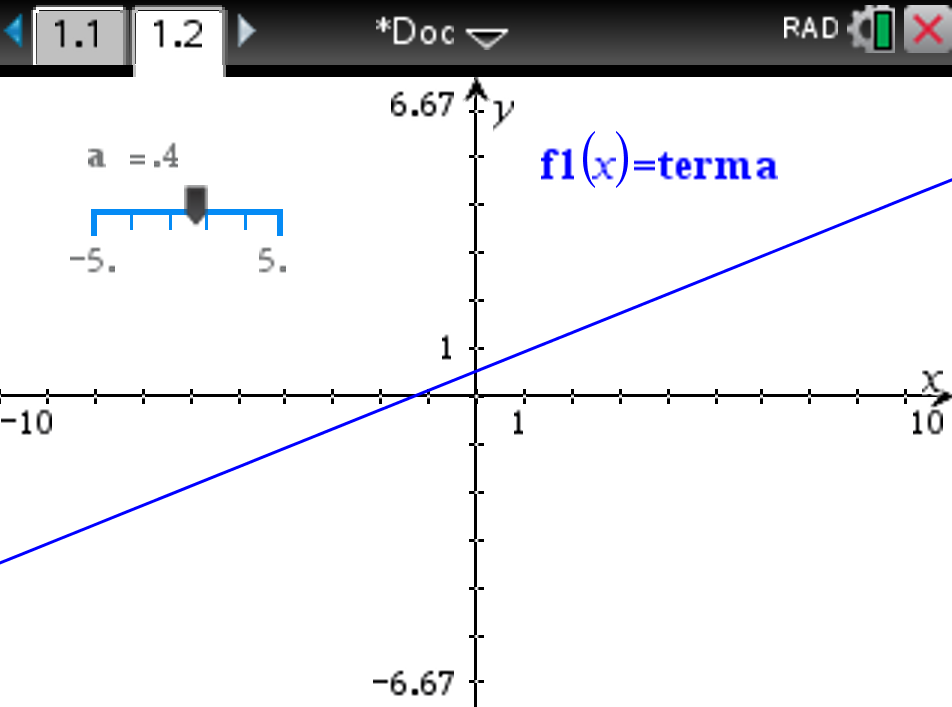
\includegraphics[width=6cm]{img/LineareFunktionTR_terma.png}}
%  \end{center}


\paragraph{Frage 1} Bei welchem Parameter $b$ hat die folgende Gleichung für $x$ die Lösung $1.5$?
$$-2x + b = 0$$

\noTRAINER{$$.....................................$$}
\TRAINER{$$b = 3$$}
Dies lösen wir, indem wir die gesuchte Lösung für $x$ einsetzen und nach $b$ auf"|lösen. Graphisch kann dies auch mit dem CAS-Rechner \textit{gelöst} werden. Definieren Sie «termb := $-2\cdot{}x+b$» und zeichnen Sie den Graphen in einer Graph-Page.
Erstellen Sie einen «Slider»\index{Slider}\index{Schieberegler} für $b$ und ziehen Sie an
diesem \textit{Slider}, bis der Wert der Geraden auf der $x$-Achse den
Wert 1.5 (gesuchte Lösung) angenähert hat.


\paragraph{Frage 2} Bei welchem Parameter $a$ hat die folgende Gleichung für $x$ die Lösung $1.5$?
$$ax-3=0$$

\noTRAINER{$$.....................................$$}
\TRAINER{$$a=2$$}
Dies nähern wir auch mit dem CAS-Rechner an. Definieren Sie den Term
$terma$ neu ($terma := a\cdot{}x-3$) und zeichnen Sie den Graphen in einer Graph-Page.
Ziehen Sie am \textit{Slider}, bis der Wert der Geraden auf der
$x$-Achse dem Wert 1.5 (gesuchte Lösung) genug nahe kommt.
}




%%\TRAINER{Aufg 247 l aus \cite{frommenwiler17alg}}
\subsection{Vorzeigeaufgabe}

\TALS{
  $$\frac{x}{n} + a - \frac{x}{m} + b = mx + c$$
\TNTeop{
  1. Alle $x$ nach links, alle «nicht $x$» nach rechts:

  $$\frac{x}{d}-\frac{x}{m}-mx = c-a-b$$

  2. $x$ ausklamern:

  $$x\left(\frac1n-\frac1m-m\right)=c-a-b$$

  3. durch die Klammer teilen

  $$x=\frac{c-a-b}{\frac1n-\frac1m-m} = (\text{optional}) = \frac{mn(c-a-b)}{m-n-m^2n}$$

}%% END TNT
}%% END TALS

\GESO{
  $$x^2 - \sqrt{2} - c = (b-x)\cdot{}(-\sqrt{5}-x)$$

  \TNTeop{
  Termumformung: $x^2-\sqrt{2} - c = -\sqrt{5}b -bx +x\sqrt{5} + x^2$\\
  beidseitig $-x^2$: $\Rightarrow -\sqrt{2}-c=-\sqrt{5}b-bx+x\sqrt{5}$\\
  Alle $x$ nach links (Rest nach rechts): $\Rightarrow bx-\sqrt{5}x= -\sqrt{5}b+\sqrt{2} + c$\\
  $x$ ausklammern: $\Rightarrow x(b-\sqrt{5})=-\sqrt{5}b+\sqrt{2} + c$\\
  $: (b-\sqrt{5})$ : $\Rightarrow x = \frac{-\sqrt{5}b+\sqrt{2} + c}{b-\sqrt{5}}$\\%%

}%% END TNT
}%% END GESO
\newpage

\subsection*{Aufgaben}
%%\TALS{\aufgabenFarbe{Aufgaben: \cite{frommenwiler17alg} S. 89, Aufg. 246. a) 247. a) c) g) 248. a) d) i) 249.}}

%%\TALS{Textaufgaben: \cite{frommenwiler17alg} S. 89 Aufg. 253}

\GESO{\olatLinkArbeitsblatt{Lineare
    Gleichungen}{https://olat.bms-w.ch/auth/RepositoryEntry/6029794/CourseNode/110662976644490}{Aufgabe
    3. und 4.}}
\TALS{\olatLinkArbeitsblatt{Lineare Gleichungen}{https://olat.bms-w.ch/auth/RepositoryEntry/6029786/CourseNode/110662976730861
}{Aufgabe 3., 4. und 5.}}


%\AadBMTA{128ff}{ 7. b) c) a) e),
%  8. a) d) e) f),
%  9. a) b) c) e) f),
%  10. a) b)
%\TALS{, 11. b) und 12. a) d) e)}
%}%% end AadBMTA

\olatLinkGESOKompendium{2.1.3.}{11}{12. bis 16.}

Testen Sie Ihr Können:

\GESO{\olatLinkArbeitsblatt{Lineare
    Gleichungen}{https://olat.bms-w.ch/auth/RepositoryEntry/6029794/CourseNode/110662976644490}{Aufgabe 6.}}
\TALS{\olatLinkArbeitsblatt{Lineare Gleichungen}{https://olat.bms-w.ch/auth/RepositoryEntry/6029786/CourseNode/110662976730861
}{Aufgabe 6.}}



\newpage
}

\TALS{\subsection{Vektoren im Taschenrechner}\index{Taschenrechner!Vektorgeometrie}

\subsubsection{Eingabe}
Vektoren im Taschenrechner werden entweder mit eckigen Klammern und
einem Strichpunkt (Semikolon) wie folgt eingegeben:
$$a := [3; 1]$$
oder direkt mit dem Vektor-Befehl bei den mathematischen Symbolen:

\bbwCenterGraphic{10cm}{tals/vecg1/img/TR_eingabe.png}

\subsubsection{Vektoraddition, Vektorsubtraktion}
Vektoren können mit $+$ bzw. $-$ addiert bzw. subtrahiert
werden:
\bbwCenterGraphic{3cm}{tals/vecg1/img/TR_plusminus.png}

\subsubsection{Gegenvektor}
Der Gegenvektor wird mit einem Minuszeichen erzeugt:
$$a:=\left(3\atop 1\right) \Longrightarrow -a = \left( -3 \atop
-1\right)$$
\newpage

\subsubsection{Mulitplikation mit Skalar (Vielfaches)}\index{Skalare Multiplikation!Taschenrechner}\index{Multiplikation!mit Skalar (TR)}

Um einen Vektor mit einem Skalar zu multiplizieren, wird beim
Taschenrechner das übliche Multiplikationszeichen verwendet.

\bbwCenterGraphic{3cm}{tals/vecg1/img/TR_skalarmultiplikation.png}

\subsection*{Aufgaben}
\AadBMTG{264}{27. a) bis e) [ohne f)]}
\newpage


\subsection{Länge im kartesischen Koordinatensystem}

Die Länge der Vektoren wird mittels «Pythagoras» berechnet.

Sei $\vec{a}  = \Spvek{x_a;y_a}$. Somit ist die Länge von
    $\vec{a}$ wie folgt zu berechnen:

    \begin{gesetz}{Betrag, Länge}{}
      Betrag von $\vec{a}$ := Länge von $\vec{a}$

      $$a = |\vec{a}| = \sqrt{x_a^2 + y_a^2}$$
      \end{gesetz}
    Notationen:

    \begin{beispiel}{}{}
      $$ \vec{a}= \Spvek{3;1}$$
        $$|\vec{a}| = \LoesungsRaumLang{\sqrt{3^2+1^2} = \sqrt{10}\approx 3.162}$$
      \end{beispiel}
    

    \begin{bemerkung}{}{}
      Im Taschenrechner werden die Vektoren mit eckigen Klammern
      definiert:

      \texttt{a := [3; 1]}

      Die Länge (Betrag) wird mit dem Befehl \texttt{norm} ermittelt:

      \texttt{norm(a)}
    \end{bemerkung}
    \subsection*{Aufgaben}
    \TALSAadBMTG{262ff}{9., 10., 19. a) 20. A, 21. a), 38.}
\newpage

\newpage

\subsubsection{Linearkombination finden}\index{Linearkombination!Taschenrechner}
Will ich einen Vektor mittels Linearkombination
\totalref{linearkombination} zerlegen, so geschieht das einfach mit dem
«solver». Bei gegebenen Vektoren $\vec{a}$, $\vec{b}$ und $\vec{c}$ sei also
wieder $s$ und $t$ gesucht, so dass gilt:
$$\vec{c} = s\cdot{}\vec{a} + t\cdot{}\vec{b}$$

\bbwCenterGraphic{90mm}{tals/vecg1/img/TR_linearkombination.png}

\subsection*{Aufgaben}
\AadBMTG{264}{27. f), 40. a) b), 42. 43. a) c)}

\newpage


Algebraisch kann man auch zeigen, dass eine Zerlegung in zwei Vektoren
nicht immer möglich ist:
\TNTeop{
Begründung Gleichungssystem:
  
  $$\vec{c} = t\cdot{}\vec{a\vphantom{b}} + s\cdot{}\vec{b}$$ heißt:
  \gleichungZZ{c_x}{t\cdot{}a_x + s\cdot{}b_x}{c_y}{t\cdot{}a_y +
    s\cdot{}b_y}

  Die Lösung (\zB mittels Einsetz-Verfahren) ist

%%  $$\det{} = a_xb_y - a_yb_x$$

  $$s = \frac{a_xc_y - a_yc_x}{a_xb_y-a_yb_x}$$
  und
  $$t = \frac{b_yc_x - b_xc_y}{a_xb_y-a_yb_x}$$

  Ist der Nenner Null, so gibt es keine (oder keine
  eindeutige) Zerlegung.
}%% END TNTeop
%%\newpage
}
\GESO{\subsection{Vektoren im Taschenrechner}\index{Taschenrechner!Vektorgeometrie}

\subsubsection{Eingabe}
Vektoren im Taschenrechner werden entweder mit eckigen Klammern und
einem Strichpunkt (Semikolon) wie folgt eingegeben:
$$a := [3; 1]$$
oder direkt mit dem Vektor-Befehl bei den mathematischen Symbolen:

\bbwCenterGraphic{10cm}{tals/vecg1/img/TR_eingabe.png}

\subsubsection{Vektoraddition, Vektorsubtraktion}
Vektoren können mit $+$ bzw. $-$ addiert bzw. subtrahiert
werden:
\bbwCenterGraphic{3cm}{tals/vecg1/img/TR_plusminus.png}

\subsubsection{Gegenvektor}
Der Gegenvektor wird mit einem Minuszeichen erzeugt:
$$a:=\left(3\atop 1\right) \Longrightarrow -a = \left( -3 \atop
-1\right)$$
\newpage

\subsubsection{Mulitplikation mit Skalar (Vielfaches)}\index{Skalare Multiplikation!Taschenrechner}\index{Multiplikation!mit Skalar (TR)}

Um einen Vektor mit einem Skalar zu multiplizieren, wird beim
Taschenrechner das übliche Multiplikationszeichen verwendet.

\bbwCenterGraphic{3cm}{tals/vecg1/img/TR_skalarmultiplikation.png}

\subsection*{Aufgaben}
\AadBMTG{264}{27. a) bis e) [ohne f)]}
\newpage


\subsection{Länge im kartesischen Koordinatensystem}

Die Länge der Vektoren wird mittels «Pythagoras» berechnet.

Sei $\vec{a}  = \Spvek{x_a;y_a}$. Somit ist die Länge von
    $\vec{a}$ wie folgt zu berechnen:

    \begin{gesetz}{Betrag, Länge}{}
      Betrag von $\vec{a}$ := Länge von $\vec{a}$

      $$a = |\vec{a}| = \sqrt{x_a^2 + y_a^2}$$
      \end{gesetz}
    Notationen:

    \begin{beispiel}{}{}
      $$ \vec{a}= \Spvek{3;1}$$
        $$|\vec{a}| = \LoesungsRaumLang{\sqrt{3^2+1^2} = \sqrt{10}\approx 3.162}$$
      \end{beispiel}
    

    \begin{bemerkung}{}{}
      Im Taschenrechner werden die Vektoren mit eckigen Klammern
      definiert:

      \texttt{a := [3; 1]}

      Die Länge (Betrag) wird mit dem Befehl \texttt{norm} ermittelt:

      \texttt{norm(a)}
    \end{bemerkung}
    \subsection*{Aufgaben}
    \TALSAadBMTG{262ff}{9., 10., 19. a) 20. A, 21. a), 38.}
\newpage

\newpage

\subsubsection{Linearkombination finden}\index{Linearkombination!Taschenrechner}
Will ich einen Vektor mittels Linearkombination
\totalref{linearkombination} zerlegen, so geschieht das einfach mit dem
«solver». Bei gegebenen Vektoren $\vec{a}$, $\vec{b}$ und $\vec{c}$ sei also
wieder $s$ und $t$ gesucht, so dass gilt:
$$\vec{c} = s\cdot{}\vec{a} + t\cdot{}\vec{b}$$

\bbwCenterGraphic{90mm}{tals/vecg1/img/TR_linearkombination.png}

\subsection*{Aufgaben}
\AadBMTG{264}{27. f), 40. a) b), 42. 43. a) c)}

\newpage


Algebraisch kann man auch zeigen, dass eine Zerlegung in zwei Vektoren
nicht immer möglich ist:
\TNTeop{
Begründung Gleichungssystem:
  
  $$\vec{c} = t\cdot{}\vec{a\vphantom{b}} + s\cdot{}\vec{b}$$ heißt:
  \gleichungZZ{c_x}{t\cdot{}a_x + s\cdot{}b_x}{c_y}{t\cdot{}a_y +
    s\cdot{}b_y}

  Die Lösung (\zB mittels Einsetz-Verfahren) ist

%%  $$\det{} = a_xb_y - a_yb_x$$

  $$s = \frac{a_xc_y - a_yc_x}{a_xb_y-a_yb_x}$$
  und
  $$t = \frac{b_yc_x - b_xc_y}{a_xb_y-a_yb_x}$$

  Ist der Nenner Null, so gibt es keine (oder keine
  eindeutige) Zerlegung.
}%% END TNTeop
%%\newpage
}

\newpage


\TALS{\subsection{Fallunterscheidung}
Einstiegsbeispiel: Ein Ball wird mit 30 m/s senkrecht nach oben geworfen.
Die Höhe kann wie folgt berechnet werden:

$$h(t)  = v_0 \cdot{} t -\frac{g}{2}\cdot{}t^2$$
Dabei ist $g$ die «Fallbeschleunigung»: $g\approx
9.8\,\frac{\text{m}}{\text{s}} / \text{ s}\, \approx 10$.

Mit Zahlen:

$$h(t) = 30\cdot{} t - \frac{10}2 \cdot{} t^2$$

Mit unseren bekannten Variablen:
$$h = 30x - 5x^2$$

Skizzieren Sie mit 
$y=h(t)$ in 10 m Schritten, $x=t$ Zeit in s:

\bbwGraph{-1}{10}{-1}{5}{
  \TRAINER{
      \bbwFunc{-0.5*(\x-3)*(\x-3)+4.5}{0:6}   
%%    \bbwFunc{-18*(\x-0.5)*(\x-0.5)+4.5){0:1}
    }
}%% end bbwGraph

\newpage

Wann ist der Ball 25 m hoch? Wann ist der Ball $h$ Meter hoch?

\TNTeop{
$$25 = 30x - 5x^2$$
  $$5x^2 - 30x + 25 = 0$$
  $$x^2 -6x + 5 = 0 \Longleftrightarrow (x-5)(x-1) = 0$$
  $$\lx=\{1 \text{ s } , 5 \text{ s }\}$$

  
  Je nach Höhe ergibt sich eine andere Anzahl der Lösungen für die Zeit:


  $$h = 30x - 5x^2 \Longleftrightarrow -5x^2 + 30x - h = 0$$

  Ist die Diskriminante = 0, so haben wir genau eine Lösung für die Zeit

  $$D = 30^2 - 4\cdot{} (-5) \cdot{} (-h) = 900 - 20h$$



  a) Berechnen $h$ für $D=0$  :

  $900 - 20h = 0 \Longrightarrow h = 45$

  b) was bedeutet dies? Bei $h=45$ Metern hat die Gleichung genau eine Lösung: Da ist der Ball ganz oben.
  $$h = 45 = 30x - 5x^2\,\,\,\, | : 5$$ 
  $$9 = 6x-x^2$$
  sortieren
  $$x^2 - 6x + 9 = 0$$
  $$(x-3)^2 = 0$$
  Nur eine Lösung, nämlich $x=t=3$ s.
  
  }%% end TNT



\newpage

Aus den Strukturaufgaben:


\aufgabenFarbe{Berechnen Sie die Lösung für $x\in\mathbb{R}$ in Abhängigkeit von $k$ mit einer vollständigen Fallunterscheidung für alle Parameterwerte $k\in\mathbb{R}$.
}

$$kx^2 - x^2 + 3x = 2$$

\TNTeop{

  \begin{tabular}{c|c|c}
    A & B & C  \\\hline
    $k-1$ & $3$ & $-2$ 
    \end{tabular}

    $$D = 9-4\cdot{} (k-1)\cdot{}(-2)$$
    $$D = 9 + 8(k-1) = 8k + 1$$
Allgemeine Lösung:
    $$x_{1,2} = \frac{-3 \pm \sqrt{8k+1}}{2k-2}$$

 1. Sonderfall Nenner: $k=1$ ist nicht möglich.

    Mit $k-1$ reduziert sich die ursprüngliche Gleichung jedoch auf:
    $$ 3x = 2 \Longrightarrow x = \frac23$$

2. Sonderfall: Diskriminante = 0:
Das heißt $8k+1=0$ und somit ist $k=\frac{-1}8$.

Somit erhalten wir für $x$ eingesetzt in die allgemeine Lösung nur noch eine Lösung:

$$x = \frac{-3\pm\sqrt{0}}{2\cdot{}\left(\frac{-1}{8} - 1\right)} = \frac43$$

3. Sonderfall: Diskriminante ist kleiner als 0:

$$8k+1 < 0 \Longleftrightarrow k <\frac{-1}8  \Longrightarrow  \lx=\{\}$$

Abgesehen von den Sonderfällen $k=1$ und $k<\frac{-1}8$ gilt die allgemeine Lösung.
    

    
    
}%% end TNT eop
%% \newpage implicit  


\subsection*{Aufgaben}

\olatLinkArbeitsblatt{GlQuad}{https://olat.bms-w.ch/auth/RepositoryEntry/6029786/CourseNode/111365560138736}{Aufgabe 13.}
}
\newpage
\TALS{\subsection{Substitution}\index{Substitution!Gleichungssysteme}\index{Lineare Gleichungssysteme!mit Substitutionsmethode}
Manchmal gibt es Situationen, in denen ein Gleichungssystem besser mit
einer Ersetzung (Substitution) als mit sturem Ausmultiplizieren gelöst
werden kann.

Betrachten Sie einmal das folgende Gleichungssystem:

\gleichungZZ{\frac{2a}{3+b} - \frac{b}{5-a}}{1}{\frac{3a}{b+3} + \frac{2b}{5-a}}{19}

Es ist offensichtlich, dass die Terme $\frac{a}{3+b}$ und
$\frac{b}{5-a}$ mehrfach vorkommen.

Hier bietet sich eine Ersetzung (Substitution) an:

$$X := \LoesungsRaum{\frac{a}{3+b}}$$

und

$$Y := \LoesungsRaum{\frac{b}{5-a}}$$

Das neue entstandene Gleichungssystem ist viel übersichtlicher und
auch einfacher zu lösen:

\TNT{2.4}{\gleichungZZ{2X - Y}{1}{3X+2Y}{19}}

Nach dem Auf"|lösen (\zB Taschenrechner) erhalten wir $X=\LoesungsRaum{3}$ bzw. $Y=\LoesungsRaum{5}$. Mit diesen Werten
können wir $a$ bzw. $b$ bestimmen.
\newpage

\textbf{Rücksubstitution}\index{Rücksubstitution}\,\\

\vspace{1mm}

\TNT{10.8}{

  \gleichungZZ{3}{\frac{a}{3+b}}{5}{\frac{b}{5-a}}

    und somit:

\gleichungZZ{9+3b}{a}{25-5a}{b}

...sortieren...

\gleichungZZ{a-3b}{9}{5a+b}{25}

Nach dem Auf"|lösen erhalten wir:

$$\mathbb{L}_{(a;b)} = \left\{ \left(\frac{21}{4} ;  -\frac{5}{4} \right)  \right\}$$
}%% END TNT


\subsection*{Aufgaben}
\TALSAadBMTA{127ff}{390. b), 391.}
\GESOAadBMTA{152}{12. c), 13. a)}
\olatLinkGESOKompendium{2.2.2}{14}{33. bis 34.}
}
\newpage

\subsection{Welches Verfahren (optional)}
Wann soll welches Verfahren eingesetzt werden? Dies ist eine
individuelle Fragestellung. Je mehr Erfahrung man hat, umso eher sieht
man die Spezialfälle. Die ABC-Formel funktioniert immer, doch
die anderen Verfahren (Binome, weitere Spezialfälle, Taschenrechner)
sind oft sinnvoller. Hier ein Versuch eines Überblicks:

\begin{rezept}{Welches Verfahren}{}

\GESO{
\begin{tabular}{|p{30mm}|p{53mm}|p{64mm}|}
	\hline
	Spezialfall $b=0$               & $5x^2 = 3$                   & Durch 5 dividieren, dann positive und negative Wurzel ziehen.\\
	\hline
	Spezialfall $c=0$               & $3x^2 = 5x$                   & Fallunterscheidung $x = 0$ und $x \ne 0$\\
	\hline
	quadratische Form            & $(x-2)^2 = 49$ & $\pm\sqrt{}$: \hspace{3mm}  $x-2=\pm 7$\\
	\hline
	faktorisiert       & $(x-4.6 + b)\cdot{}(x+a) = 0$ & Lösungen hier $x_1=4.6-b$ und $x_2 = -a$\\
	\hline
	Einfache Zahlen            & $x^2 -2x + 1= 0$           & ABC-Formel (Mitternachtsformel) oder faktorisieren $x^2-2x+1=(x-1)^2$ und danach jeden einzelnen Faktor $=0$ setzen.\\
	\hline
	Komplizierte Zahlen        & $7.3x^2 - 8x - 3.4 = 0$       & Taschenrechner \tiprobutton{cos_poly-solv}             \\
	\hline
%	Variable (Parameter)       & $7.3x^2 - cx + 2.6=0$         & ABC-Formel (Mitternachtsformel) \\
%	\hline
\end{tabular}
\newpage
}

\TALS{
\begin{tabular}{|p{35mm}|p{53mm}|p{60mm}|}
	\hline
	Spezialfall $b=0$               & $5x^2 = 3$                   & Durch 5 dividieren, dann positive und negative Wurzel ziehen.\\
	\hline
	Spezialfall $c=0$               & $3x^2 = 5x$                   & Fallunterscheidung $x = 0$ und $x \ne 0$\\
	\hline
	quadratische Form            & $(x-2)^2 = 49$ & $\pm\sqrt{}$: \hspace{3mm}  $x-2=\pm 7$\\
  \hline
	faktorisiert & $(x-4.6 + b)\cdot{}(x+a) = 0$ & Lösungen hier $x_1=4.6-b$ und $x_2 = -a$\\
	\hline
	Einfache Zahlen      & $6x^2 -3x - 18 = 0$               & ABC-Formel (Mitternachtsformel) \\
	\hline
	Komplizierte Zahlen  & $7.3x^2 - 8x - 3.4 = 0$           & Taschenrechner (solve())                \\
	\hline
	Variable (Parameter) & $7.3x^2 - cx + 2.6=0$         & Taschenrechner                          \\
	\hline
	Anzahl Lösungen auf eine beschränken & $7.3x^2 - cx + 2.6 = 	0$     & 	Diskriminante mit Taschenrechner Null setzen.\\
	\hline
\end{tabular} 
}

\end{rezept}

\subsection*{Aufgaben}

\GESO{\olatLinkArbeitsblatt{GlQuad}{https://olat.bms-w.ch/auth/RepositoryEntry/6029794/CourseNode/111365559999287}{Aufgabe
15. Bsp. a) c) e) g) j) l) n)}
}%% end GESO

\TALS{\olatLinkArbeitsblatt{GlQuad}{https://olat.bms-w.ch/auth/RepositoryEntry/6029786/CourseNode/111365560138736}{Aufgabe
15. Auswahl: a) c) e) h) l) n) q)}
}%% end TALS

\newpage
